\documentclass[11pt,a4paper,]{article}
\usepackage{lmodern}

\usepackage{amssymb,amsmath}
\usepackage{ifxetex,ifluatex}
\usepackage{fixltx2e} % provides \textsubscript
\ifnum 0\ifxetex 1\fi\ifluatex 1\fi=0 % if pdftex
  \usepackage[T1]{fontenc}
  \usepackage[utf8]{inputenc}
\else % if luatex or xelatex
  \usepackage{unicode-math}
  \defaultfontfeatures{Ligatures=TeX,Scale=MatchLowercase}
\fi
% use upquote if available, for straight quotes in verbatim environments
\IfFileExists{upquote.sty}{\usepackage{upquote}}{}
% use microtype if available
\IfFileExists{microtype.sty}{%
\usepackage[]{microtype}
\UseMicrotypeSet[protrusion]{basicmath} % disable protrusion for tt fonts
}{}
\PassOptionsToPackage{hyphens}{url} % url is loaded by hyperref
\usepackage[unicode=true]{hyperref}
\hypersetup{
            pdftitle={Improving forecasts with clustering and meta data},
            pdfkeywords={hierarchical forecasting, grouped forecasting, reconciled forecast,
linear regression, \ldots{}},
            pdfborder={0 0 0},
            breaklinks=true}
\urlstyle{same}  % don't use monospace font for urls
\usepackage{geometry}
\geometry{left=2.5cm,right=2.5cm,top=2.5cm,bottom=2.5cm}
\usepackage[style=authoryear-comp,]{biblatex}
\addbibresource{references.bib}
\usepackage{longtable,booktabs}
% Fix footnotes in tables (requires footnote package)
\IfFileExists{footnote.sty}{\usepackage{footnote}\makesavenoteenv{long table}}{}
\usepackage{graphicx,grffile}
\makeatletter
\def\maxwidth{\ifdim\Gin@nat@width>\linewidth\linewidth\else\Gin@nat@width\fi}
\def\maxheight{\ifdim\Gin@nat@height>\textheight\textheight\else\Gin@nat@height\fi}
\makeatother
% Scale images if necessary, so that they will not overflow the page
% margins by default, and it is still possible to overwrite the defaults
% using explicit options in \includegraphics[width, height, ...]{}
\setkeys{Gin}{width=\maxwidth,height=\maxheight,keepaspectratio}
\IfFileExists{parskip.sty}{%
\usepackage{parskip}
}{% else
\setlength{\parindent}{0pt}
\setlength{\parskip}{6pt plus 2pt minus 1pt}
}
\setlength{\emergencystretch}{3em}  % prevent overfull lines
\providecommand{\tightlist}{%
  \setlength{\itemsep}{0pt}\setlength{\parskip}{0pt}}
\setcounter{secnumdepth}{5}

% set default figure placement to htbp
\makeatletter
\def\fps@figure{htbp}
\makeatother


\title{Improving forecasts with clustering and meta data}

%% MONASH STUFF

%% CAPTIONS
\RequirePackage{caption}
\DeclareCaptionStyle{italic}[justification=centering]
 {labelfont={bf},textfont={it},labelsep=colon}
\captionsetup[figure]{style=italic,format=hang,singlelinecheck=true}
\captionsetup[table]{style=italic,format=hang,singlelinecheck=true}

%% FONT
\RequirePackage{bera}
\RequirePackage{mathpazo}

%% HEADERS AND FOOTERS
\RequirePackage{fancyhdr}
\pagestyle{fancy}
\rfoot{\Large\sffamily\raisebox{-0.1cm}{\textbf{\thepage}}}
\makeatletter
\lhead{\textsf{\expandafter{\@title}}}
\makeatother
\rhead{}
\cfoot{}
\setlength{\headheight}{15pt}
\renewcommand{\headrulewidth}{0.4pt}
\renewcommand{\footrulewidth}{0.4pt}
\fancypagestyle{plain}{%
\fancyhf{} % clear all header and footer fields
\fancyfoot[C]{\sffamily\thepage} % except the center
\renewcommand{\headrulewidth}{0pt}
\renewcommand{\footrulewidth}{0pt}}

%% MATHS
\RequirePackage{bm,amsmath}
\allowdisplaybreaks

%% GRAPHICS
\RequirePackage{graphicx}
\setcounter{topnumber}{2}
\setcounter{bottomnumber}{2}
\setcounter{totalnumber}{4}
\renewcommand{\topfraction}{0.85}
\renewcommand{\bottomfraction}{0.85}
\renewcommand{\textfraction}{0.15}
\renewcommand{\floatpagefraction}{0.8}

%\RequirePackage[section]{placeins}

%% SECTION TITLES
\RequirePackage[compact,sf,bf]{titlesec}
\titleformat{\section}[block]
  {\fontsize{15}{17}\bfseries\sffamily}
  {\thesection}
  {0.4em}{}
\titleformat{\subsection}[block]
  {\fontsize{12}{14}\bfseries\sffamily}
  {\thesubsection}
  {0.4em}{}
\titlespacing{\section}{0pt}{*5}{*1}
\titlespacing{\section}{0pt}{*2}{*0.2}


%% TITLE PAGE
\def\Date{\number\day}
\def\Month{\ifcase\month\or
 January\or February\or March\or April\or May\or June\or
 July\or August\or September\or October\or November\or December\fi}
\def\Year{\number\year}

\makeatletter
\def\wp#1{\gdef\@wp{#1}}\def\@wp{??/??}
\def\jel#1{\gdef\@jel{#1}}\def\@jel{??}
\def\showjel{{\large\textsf{\textbf{JEL classification:}}~\@jel}}
\def\nojel{\def\showjel{}}
\def\addresses#1{\gdef\@addresses{#1}}\def\@addresses{??}
\def\cover{{\sffamily\setcounter{page}{0}
        \thispagestyle{empty}%
        \vspace*{-2cm}
        \centerline{\raisebox{-1.8cm}{
\includegraphics[width=5cm]{MBSportrait}}\hspace*{9cm} ISSN 1440-771X}\vspace{0.99cm}
        \begin{center}\Large
        Department of Econometrics and Business Statistics\\[.5cm]
        \scriptsize http://business.monash.edu/econometrics-and-business-statistics/research/publications
        \end{center}\vspace{2cm}
        \begin{center}
        \fbox{\parbox{14cm}{\begin{onehalfspace}\centering\Huge\vspace*{0.3cm}
                \textsf{\textbf{\expandafter{\@title}}}\vspace{1cm}\par
                \LARGE\@author\end{onehalfspace}
        }}
        \end{center}
        \vfill
                \begin{center}\Large
                \Month~\Year\\[1cm]
                Working Paper \@wp
        \end{center}}}
\def\pageone{{\sffamily\setstretch{1}%
        \thispagestyle{empty}%
        \vbox to \textheight{%
        \raggedright\baselineskip=1.2cm
     {\fontsize{24.88}{30}\sffamily\textbf{\expandafter{\@title}}}
        \vspace{2cm}\par
        \hspace{1cm}\parbox{14cm}{\sffamily\large\@addresses}\vspace{1cm}\vfill
        \hspace{1cm}{\large\Date~\Month~\Year}\\[1cm]
        \hspace{1cm}\showjel\vss}}}
\def\blindtitle{{\sffamily
     \thispagestyle{plain}\raggedright\baselineskip=1.2cm
     {\fontsize{24.88}{30}\sffamily\textbf{\expandafter{\@title}}}\vspace{1cm}\par
        }}
\def\titlepage{{\cover\newpage\pageone\newpage\blindtitle}}

\def\blind{\def\titlepage{{\blindtitle}}\let\maketitle\blindtitle}
\def\titlepageonly{\def\titlepage{{\pageone\end{document}}}}
\def\nocover{\def\titlepage{{\pageone\newpage\blindtitle}}\let\maketitle\titlepage}
\let\maketitle\titlepage
\makeatother

%% SPACING
\RequirePackage{setspace}
\spacing{1.5}

%% LINE AND PAGE BREAKING
\sloppy
\clubpenalty = 10000
\widowpenalty = 10000
\brokenpenalty = 10000
\RequirePackage{microtype}

%% PARAGRAPH BREAKS
\setlength{\parskip}{1.4ex}
\setlength{\parindent}{0em}

%% HYPERLINKS
\RequirePackage{xcolor} % Needed for links
\definecolor{darkblue}{rgb}{0,0,.6}
\RequirePackage{url}

\makeatletter
\@ifpackageloaded{hyperref}{}{\RequirePackage{hyperref}}
\makeatother
\hypersetup{
     citecolor=0 0 0,
     breaklinks=true,
     bookmarksopen=true,
     bookmarksnumbered=true,
     linkcolor=darkblue,
     urlcolor=blue,
     citecolor=darkblue,
     colorlinks=true}

%% KEYWORDS
\newenvironment{keywords}{\par\vspace{0.5cm}\noindent{\sffamily\textbf{Keywords:}}}{\vspace{0.25cm}\par\hrule\vspace{0.5cm}\par}

%% ABSTRACT
\renewenvironment{abstract}{\begin{minipage}{\textwidth}\parskip=1.4ex\noindent
\hrule\vspace{0.1cm}\par{\sffamily\textbf{\abstractname}}\newline}
  {\end{minipage}}


\usepackage[T1]{fontenc}
\usepackage[utf8]{inputenc}

\usepackage[showonlyrefs]{mathtools}
\usepackage[no-weekday]{eukdate}

%% BIBLIOGRAPHY

\makeatletter
\@ifpackageloaded{biblatex}{}{\usepackage[style=authoryear-comp, backend=biber, natbib=true]{biblatex}}
\makeatother
\ExecuteBibliographyOptions{bibencoding=utf8,minnames=1,maxnames=3, maxbibnames=99,dashed=false,terseinits=true,giveninits=true,uniquename=false,uniquelist=false,doi=false, isbn=false,url=true,sortcites=false}

\DeclareFieldFormat{url}{\texttt{\url{#1}}}
\DeclareFieldFormat[article]{pages}{#1}
\DeclareFieldFormat[inproceedings]{pages}{\lowercase{pp.}#1}
\DeclareFieldFormat[incollection]{pages}{\lowercase{pp.}#1}
\DeclareFieldFormat[article]{volume}{\mkbibbold{#1}}
\DeclareFieldFormat[article]{number}{\mkbibparens{#1}}
\DeclareFieldFormat[article]{title}{\MakeCapital{#1}}
\DeclareFieldFormat[article]{url}{}
%\DeclareFieldFormat[book]{url}{}
%\DeclareFieldFormat[inbook]{url}{}
%\DeclareFieldFormat[incollection]{url}{}
%\DeclareFieldFormat[inproceedings]{url}{}
\DeclareFieldFormat[inproceedings]{title}{#1}
\DeclareFieldFormat{shorthandwidth}{#1}
%\DeclareFieldFormat{extrayear}{}
% No dot before number of articles
\usepackage{xpatch}
\xpatchbibmacro{volume+number+eid}{\setunit*{\adddot}}{}{}{}
% Remove In: for an article.
\renewbibmacro{in:}{%
  \ifentrytype{article}{}{%
  \printtext{\bibstring{in}\intitlepunct}}}

\AtEveryBibitem{\clearfield{month}}
\AtEveryCitekey{\clearfield{month}}

\makeatletter
\DeclareDelimFormat[cbx@textcite]{nameyeardelim}{\addspace}
\makeatother
\renewcommand*{\finalnamedelim}{%
  %\ifnumgreater{\value{liststop}}{2}{\finalandcomma}{}% there really should be no funny Oxford comma business here
  \addspace\&\space}


\wp{no/yr}
\jel{C10,C14,C22}

\nocover

\author{Mahsa~Ashouri, Rob J~Hyndman}
\addresses{\textbf{Mahsa Ashouri}\newline
Institute of Service Science, National Tsing Hua University, Taiwan
\newline{Email: \href{mailto:mahsa.ashouri@iss.nthu.edu.tw}{\nolinkurl{mahsa.ashouri@iss.nthu.edu.tw}}}\newline Corresponding author\\[1cm]
\textbf{Rob J Hyndman}\newline
Monash University, Clayton VIC 3800, Australia
\newline{Email: \href{mailto:rob.hyndman@monash.edu}{\nolinkurl{rob.hyndman@monash.edu}}}\\[1cm]
}

\date{\sf\Date~\Month~\Year}
\makeatletter
 \lfoot{\sf Ashouri, Hyndman: \@date}
\makeatother

%% Any special functions or other packages can be loaded here.


\usepackage{amsthm}
\newtheorem{theorem}{Theorem}[section]
\newtheorem{lemma}{Lemma}[section]
\theoremstyle{definition}
\newtheorem{definition}{Definition}[section]
\newtheorem{corollary}{Corollary}[section]
\newtheorem{proposition}{Proposition}[section]
\theoremstyle{definition}
\newtheorem{example}{Example}[section]
\theoremstyle{definition}
\newtheorem{exercise}{Exercise}[section]
\theoremstyle{remark}
\newtheorem*{remark}{Remark}
\newtheorem*{solution}{Solution}
\begin{document}
\maketitle
\begin{abstract}
A brief summary of our ideas
\end{abstract}
\begin{keywords}
hierarchical forecasting, grouped forecasting, reconciled forecast,
linear regression, \ldots{}
\end{keywords}

\section{Introduction}\label{introduction}

\subsection{Hierarchical time series}\label{hierarchical-time-series}

One of the consequences of increasing internet usage and life digitizing
is increasing the amount of collected time series data. In some cases
these time series can be structured and disaggregated based on
hierarchies or groups such as geographical location and gender. One
example for hierarchical time series can be the amount of sales in
restaurant chains which can be disaggregated into different branches and
then foods or drinks. You can check a visualizing example of these time
series structure in figure @ref(fig:example of hierarchy structure). In
this example the hierarchy includes three levels. Top level, level 0, is
the total series which is the aggregation of all the bottom level
series, the middle level, level 1, series are aggregation of their own
bottom level series for instance series A is the aggregation of AA and
AB and finally the bottom level , level 2, series which includes the
most disaggregated series.

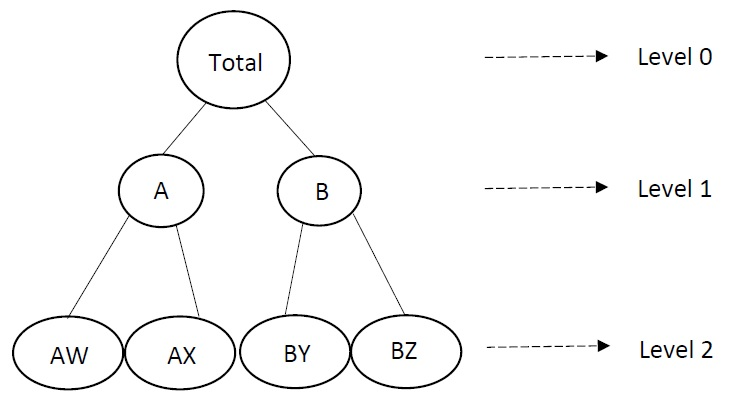
\includegraphics{Paper-Figures/hierarchical_example.jpg}\{\#fig:example
of hierarchy structure\}

\subsection{Forecasting hierarchical and grouped time
series}\label{forecasting-hierarchical-and-grouped-time-series}

For hierarchical or grouped time series ignoring the hierarchy or
grouping structure and finding forecasts for all the series can result
low accuracy level. Since the most disaggregated or bottom level series
are highly noisy and then their forecasting results are not that
accurate. On the other hand, the most aggregated or total series, is
smoother and less noisy though forecasting them is easier
\autocite{fliedner2001hierarchical}.

In literature there are some methods which consider hierarchy structure
information in forecasting time series including top-down
\autocite{gross1990disaggregation}, bottom-up
\autocite{kahn1998revisiting}, middle-out and optimal combination
\autocite{hyndman2011optima} approaches. In top-down approach we first
forecast the total series and then disaggregate the forecast to bottom
level series based on a set of historical and forecasted proportions (
details about proportions in \textcite{athanasopoulos2009hierarchical}).
In bottom-up approach the forecasts in each level of hierarchy can be
computed using aggregating the bottom level series forecast. In
middle-out approach, the process can be started from one of the middle
levels and other forecasted can be computed using aggregation for upper
levels and disaggregation for lower levels. Finally optimal combination
uses all the base forecasts, forecasts for all the series in the whole
hierarchy structure, then applies some regression models to reconcile
those base forecasts. The advantage of the latest methods in compare
with other methods is that it considers the correlation among the series
in all the levels of hierarchy.

\subsection{Challenges and
motivations}\label{challenges-and-motivations}

In optimal combination approach we need to compute the base forecast for
all the series first.

\section{Proposed approach}\label{proposed-approach}

\section{Applications}\label{applications}

In this section we are illustrating our approach and its results using
two examples, Australian domestic tourism and Wikipedia pageview
datasets. We are also comparing the forecasting accuracy levels among
our method, ETS and ARIMA with and without reconciliation effect on
forecasting.

\subsection{Australian domestic tourism
dataset}\label{australian-domestic-tourism-dataset}

This dataset is 19 years (1998-2017) quarterly and measured by
Australians visitor nights spend away from home collected each month
\autocite{wickramasuriya2018optimal}. In total this dataset includes 304
time series with length 228. The hierarchy and grouping structure for
this dataset is made using geographical and purpose information. In this
dataset we have three levels geographical division for Australia. In the
first level Australia was divided into seven `State' including New South
Wales (NSW), Victoria (VIC), Queensland (QLD), South Australia (SA),
Western Australia (WA), Tasmania (TAS) and Northern Territory (NT). In
the second and third levels its divided into 27 `Zone' and 76 `Region'
(details about Australia geographical division in Table
@ref(Australia\_geographical\_division)). Also for `Purpose' we provided
with four groups: Holiday (Hol), Visiting (Vis), Business (Bis) and
Others (Oth).

\begin{longtable}[]{@{}crccrc@{}}
\toprule
Series & Name & Lable & Series & Name & Lable\tabularnewline
\midrule
\endhead
Total & & & Region & &\tabularnewline
1 & Australia & Total & 55 & Lakes & BCA\tabularnewline
State & & & 56 & Gippsland & BCB\tabularnewline
2 & NSW & A & 57 & Phillip Island & BCC\tabularnewline
3 & VIC & B & 58 & General Murray & BDA\tabularnewline
4 & QLD & C & 59 & Goulburn & BDB\tabularnewline
5 & SA & D & 60 & High Country & BDC\tabularnewline
6 & WA & E & 61 & Merbourne East & BDD\tabularnewline
7 & TAS & F & 62 & Upper Yarra & BDE\tabularnewline
8 & NT & G & 63 & Murray East & BDF\tabularnewline
Zone & & & 64 & Wimmera+Mallee & BEA\tabularnewline
9 & Metro NSW & AA & 65 & Western Grampians & BEB\tabularnewline
10 & Nth Coast NSW & AB & 66 & Bendigo Loddon & BEC\tabularnewline
11 & Sth Coast NSW & AC & 67 & Macedon & BED\tabularnewline
12 & Sth NSW & AD & 68 & Spa Country & BEE\tabularnewline
13 & Nth NSW & AE & 69 & Ballarat & BEF\tabularnewline
14 & ACT & AF & 70 & Central Highlands & BEG\tabularnewline
15 & Metro VIC & BA & 71 & Gold Coast & CAA\tabularnewline
16 & West Coast VIC & BB & 72 & Brisbane & CAB\tabularnewline
17 & East Coast VIC & BC & 73 & Sunshine Coast & CAC\tabularnewline
18 & Nth East VIC & BD & 74 & Central Queensland & CBA\tabularnewline
19 & Nth West VIC & BE & 75 & Bundaberg & CBB\tabularnewline
20 & Metro QLD & CA & 76 & Fraser Coast & CBC\tabularnewline
21 & Central Coast QLD & CB & 77 & Mackay & CBD\tabularnewline
22 & Nth Coast QLD & CC & 78 & Whitsundays & CCA\tabularnewline
23 & Inland QLD & CD & 79 & Northern & CCB\tabularnewline
24 & Metro SA & DA & 80 & Tropical North Queensland & CCC\tabularnewline
25 & Sth Coast SA & DB & 81 & Darling Downs & CDA\tabularnewline
26 & Inland SA & DC & 82 & Outback & CDB\tabularnewline
27 & West Coast SA & DD & 83 & Adelaide & DAA\tabularnewline
28 & West Coast WA & EA & 84 & Barrosa & DAB\tabularnewline
29 & Nth WA & EB & 85 & Adelaide Hills & DAC\tabularnewline
30 & Sth WA & EC & 86 & Limestone Coast & DBA\tabularnewline
31 & Sth TAS & FA & 87 & Fleurieu Peninsula & DBB\tabularnewline
32 & Nth East TAS & FB & 88 & Kangaroo Island & DBC\tabularnewline
33 & Nth West TAS & FC & 89 & Murraylands & DCA\tabularnewline
34 & Nth Coast NT & GA & 90 & Riverland & DCB\tabularnewline
35 & Central NT & GB & 91 & Clare Valley & DCC\tabularnewline
Region & & & 92 & Flinders Range and Outback & DCD\tabularnewline
36 & Sydney & AAA & 93 & Eyre Peninsula & DDA\tabularnewline
37 & Central Coast & AAB & 94 & Yorke Peninsula & DDB\tabularnewline
38 & Hunter & ABA & 95 & Australia's Coral Coast & EAA\tabularnewline
39 & North Coast NSW & ABB & 96 & Experience Perth & EAB\tabularnewline
40 & Northern Rivers Tropical NSW & ABC & 97 & Australia's SouthWest &
EAC\tabularnewline
41 & South Coast & ACA & 98 & Australia's North West &
EBA\tabularnewline
42 & Snowy Mountains & ADA & 99 & Australia's Golden Outback &
ECA\tabularnewline
43 & Capital Country & ADB & 100 & Hobart and the South &
FAA\tabularnewline
44 & The Murray & ADC & 101 & East Coast & FBA\tabularnewline
45 & Riverina & ADD & 102 & Launceston, Tamar and the North &
FBB\tabularnewline
46 & Central NSW & AEA & 103 & North West & FCA\tabularnewline
47 & New England North West & AEB & 104 & Wilderness West &
FCB\tabularnewline
48 & Outback NSW & AEC & 105 & Darwin & GAA\tabularnewline
49 & Blue Mountains & AED & 106 & Kakadu Arnhem & GAB\tabularnewline
50 & Canberra & AFA & 107 & Katherine Daly & GAC\tabularnewline
51 & Melbourne & BAA & 108 & Barkly & GBA\tabularnewline
52 & Peninsula & BAB & 109 & Lasseter & GBB\tabularnewline
53 & Geelong & BAc & 110 & Alice Springs & GBC\tabularnewline
54 & Western & BBA & 111 & MacDonnell & GBD\tabularnewline
\bottomrule
\end{longtable}

\subsection{Wikipedia pageview
dataset}\label{wikipedia-pageview-dataset}

The second dataset is one year daily data (2016-06-01 to 2017-06-29)
consists of a collection of Wikipedia pageviews time series for the most
popular social networks articles \autocite[.]{Ashouri}. Its grouping
attributes are `Agent': Spider, User, `Access': Desktop, Mobile app,
Mobile web, `Purpose': Blogging related, Business, Gaming, General
purpose, Life style, Photo sharing, Reunion, Travel, Video and
`Language': en (English), de (German), es (Spanish), zh (Chinese). The
final dataset includes 913 time series, each with length 394.

\section{Conclusion}\label{conclusion}

\printbibliography[title=Discussion and further research]

\end{document}
